\documentclass[../thesis.tex]{subfiles}
\section{Contagion on the Model}

Now that the groundwork has been layed down, we can focus on the object of our inquiry: demand shocks and price contagions. As equation (\ref{local_p_comp}) shows, price contagion depends, via $P(\matr{Y})$, linearly on the matrix $(2\I + \G)^{-1}$. We can call this the ``bargaining power'' matrix, since it allocates the excess revenues, $\Delta_t$, among providers in the network. For example, in the case of a positive demand shock and an increase in the local price of electricity of a given node, the excess demand will be partially absorbed by all other nodes in the network which, in turn, causes a contagion of local price hikes. Hence, the spread of the price hikes depends on the bargaining power of nodes in the matrix. Sticking with our example, if $X_{i, t}$ increases suddenly, $\Delta^{(i, j)}_t$ increases, and the cross-border price on another edge $(k, l)$ increases by

\begin{equation*}
  (2\I + \G)^{-1}_{(k, l), (i, j)}.
\end{equation*}

This implies that a provider with a stronger bargaining position reacts more strongly to price changes, captures higher revenue, which leads to higher prices in the local market. Hence a more equal distribution of bargaining power leads to lower revenues for providers and lower price hikes. To formalize this, consider the entry $(i, j)$ in $P(\Y_t)$

\begin{equation*}
  P^{(i, j)}_t = \frac{\sum_{(l, m) \in E} \Delta^{(l, m)}_t \  (2\I + \G)^{-1}_{(i, j), (l, m)}}{Y^{(i, j)}_t},
\end{equation*} where $\sum_{(l, m) \in E}$ is a summation over the row $(i, j)$ of $(2\I + \G)^{-1}$. Now assume there is some demand shock in a node $k$. We would like to understand the effect this has on prices today, $P^{(i, j)}_t$. The derivative of the price today with respect to demand today yields,

\begin{equation*}
  \begin{split}
    \frac{\partial P^{(i, j)}_{t}}{\partial X_{k, t}}
    &= \frac{1}{Y^{(i, j)}_t} \left( p_{k, t} \  \sum_{(k, m) \in E} (2\I + \G)^{-1}_{(i, j), (k, m)} - p_{k, t} \  \sum_{(l, k) \in E} (2\I + \G)^{-1}_{(i, j), (l, k)} \right) - \frac{P^{(i, j)}_t}{ Y_t^{(i, j)}} \\
    &= \frac{p_{k, t}}{Y^{(i, j)}_t} \underbrace{\left(\sum_{(k, m) \in E} (2\I + \G)^{-1}_{(i, j), (k, m)} -  \sum_{(l, k) \in E} (2\I + \G)^{-1}_{(i, j), (l, k)} \right)}_{\text{bargaining power of $k$ on the network}} - \frac{P^{(i, j)}_t}{ Y_t^{(i, j)}}.
  \end{split}
\end{equation*}

This bargaining power value gives a first order approximation of the effect on the network of a demand shock in a given node. In Figure \ref{fig:influence} I plotted the bargaining power of each node on different graphs that will be used in the simulation. It is wise to stop here with the analytical work on an arbitrary graph $\mathcal{A}$ given the complex behavior of $\partial P^{(i, j)}_{t + 1} / \partial X_{k, t}$. In the next section I will look at contagion by picking some simple examples, working out the core structure and bargaining power analytically, and then simulating the systems' behavior.

\begin{figure}[H]
  \centering
  % First row
  \begin{subfigure}[t]{.3\textwidth}
    \centering
    \includegraphics[width=\linewidth]{\bargpath/line.pdf}
    \caption{On a path graph} \label{fig:linepower}
  \end{subfigure}
  \hfill
  \begin{subfigure}[t]{.3\textwidth}
    \centering
    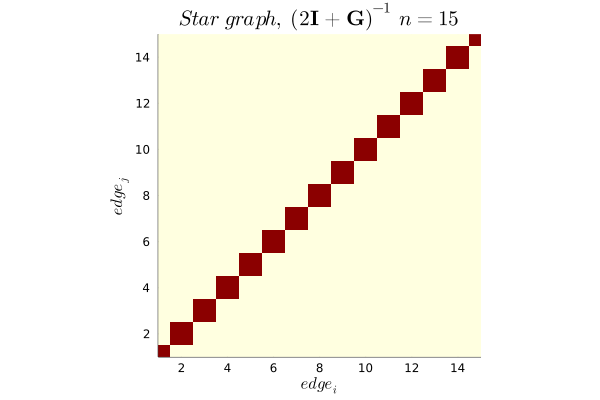
\includegraphics[width=\linewidth]{\bargpath/star.pdf}
    \caption{On a star graph} \label{fig:starpower}
  \end{subfigure}
  % Second row
  \centering
  \begin{subfigure}[t]{.3\textwidth}
    \centering
    \includegraphics[width=\linewidth]{\bargpath/binarytree.pdf}
    \caption{On a binary tree} \label{fig:btreepower}
  \end{subfigure}
  \caption{Bargaining power over the network} \label{fig:influence}
\end{figure}

\subsection{Two providers}

\subfile{sections/examples/twoproviders.tex}

\subsection{Star and Path}

\subfile{sections/examples/starpath.tex}

